         \chapter{Safety in the laboratory}
    \setcounter{figure}{1}
    \setcounter{subfigure}{1}
    \label{m38491}
\section{ Introduction}
            \nopagebreak
            \label{m38491*cid1} $ \hspace{-5pt}\begin{array}{cccccccccccc}   \end{array} $ \hspace{2 pt}\raisebox{-5 pt}{
\includegraphics[width=0.5cm]{col11305.imgs/summary_www.png}} {(section shortcode: P10115 )} \par 
\label{m38491*id5632}A laboratory (be it for physics, chemistry or other sciences) can be a very dangerous and daunting place. However, if you follow a few simple guidelines you can safely carry out experiments in the lab without endangering yourself or others around you.
\par 
\section{ General safety rules}
            \nopagebreak
            \label{m38491*cid2} $ \hspace{-5pt}\begin{array}{cccccccccccc}   \end{array} $ \hspace{2 pt}\raisebox{-5 pt}{
\includegraphics[width=0.5cm]{col11305.imgs/summary_www.png}} {(section shortcode: P10116 )} \par 
\label{m38491*id7342}The following are some of the general guidelines and rules that you should always observe when working in a laboratory.
\label{m38491*id634222}\begin{enumerate}[noitemsep, label=\textbf{\arabic*}. ] 
            \label{m38491*id632}\item Do not eat or drink in the lab. Do not use lab glassware to eat or drink from.
\label{m38491*id6124}\item Always behave responsibly in the lab. Do not run around or play practical jokes.
\label{m38491*id6342}\item In case of accidents or chemical spills call your teacher at once.
\label{m38491*id7324}\item Always check with your teacher how to dispose of waste. Chemicals should not be disposed of down the sink.
\label{m38491*id632324}\item Only perform the experiments that your teacher instructs you to. Never mix chemicals for fun.
\label{m38491*id6242313}\item Never perform experiments alone. 
\label{m38491*id5512}\item Always check the safety data of any chemicals you are going to use. 
\label{m38491*id523465}\item Follow the given instructions exactly. Do not mix up steps or try things in a different order.
\label{m38491*id73221}\item Be alert and careful when handling chemicals, hot glassware, etc.  
\label{m38491*id5621}\item Ensure all bunsen burners are turned off at the end of the practical and all chemical containers are sealed.
\end{enumerate}
\par 
\section{ Hazard signs}
            \nopagebreak
            \label{m38491*eip-411} $ \hspace{-5pt}\begin{array}{cccccccccccc}   \end{array} $ \hspace{2 pt}\raisebox{-5 pt}{
\includegraphics[width=0.5cm]{col11305.imgs/summary_www.png}} {(section shortcode: P10117 )} \par \label{m38491*eip-990}The image below lists some of the common hazards signs that you may encounter. You should know what all of these mean.
    \setcounter{subfigure}{0}
	\begin{figure}[H] % horizontal\label{m38491*id63458}
    \begin{center}
    \label{m38491*id63458!!!underscore!!!media}\label{m38491*id63458!!!underscore!!!printimage}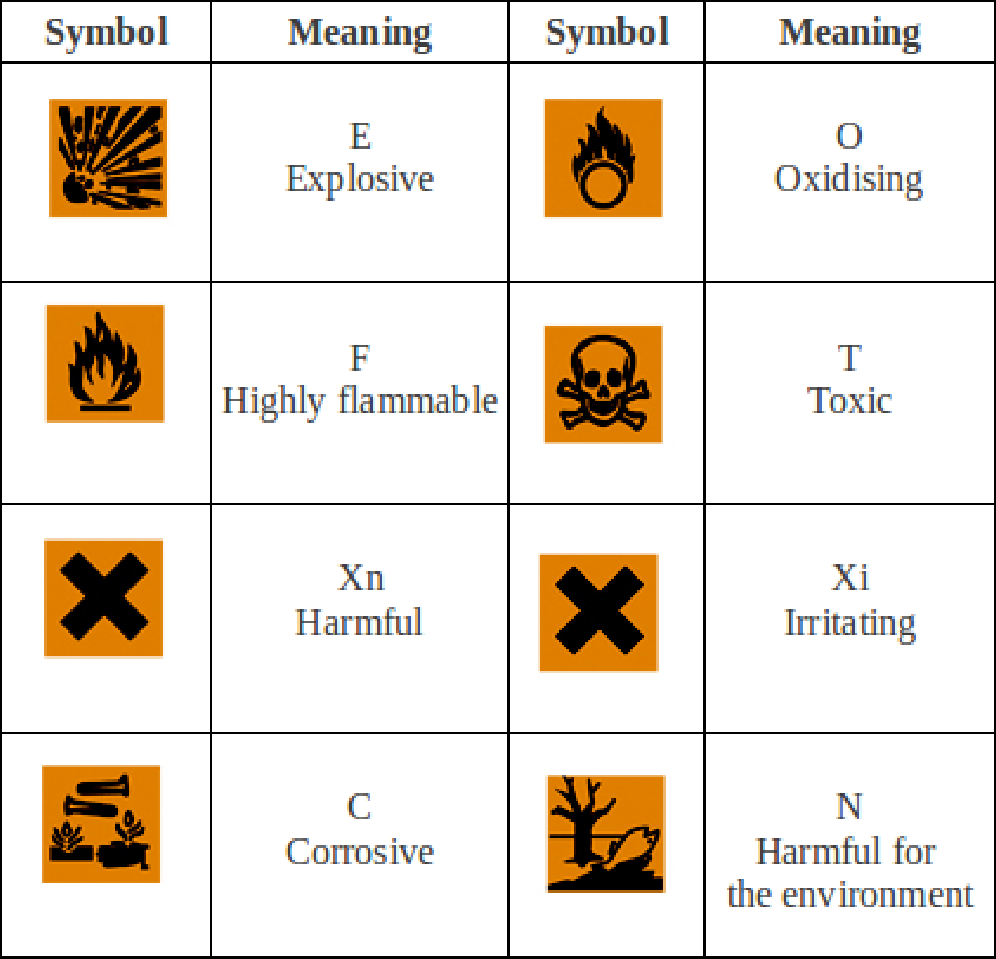
\includegraphics[width=300px]{col11305.imgs/m38491_safety.png} % m38491;safety.png;;;6.0;8.5;
      \vspace{2pt}
    \vspace{.1in}
    \end{center}
 \end{figure}       \par \section{ Notes and information}
            \nopagebreak
            \label{m38491*eip-475} $ \hspace{-5pt}\begin{array}{cccccccccccc}   \end{array} $ \hspace{2 pt}\raisebox{-5 pt}{
\includegraphics[width=0.5cm]{col11305.imgs/summary_www.png}} {(section shortcode: P10118 )} \par \label{m38491*eip-86}
You can find safety data sheets at Merck\footnote{http://www.merck-chemicals.co.za/safety-data-sheets/c\_O\_Sb.s1LQz0AAAEWVOYfVhTo}
        . You should always look at these data sheets anytime you work with a new chemical.
\par 
\label{m38491*id7322}You should always try dispose of chemicals correctly and safely. Many chemicals cannot simply be washed down the sink. 
\par 
\label{m38491**end}
      \newpage 
      \def\leftmark{GLOSSARY}
      \def\rightmark{GLOSSARY}
      \begin{indexheading}
